\section{Using distant memory in reasoning}
\label{sec:diagnostic}

RMA is what lets EdgeRock-4B use evidence beyond its local window. On 256 contexts of 16K to 130,000 input tokens, with four queries each covering retrieval, state updates, cross-document combination, and variable binding, it answers \textbf{94.1\%} of queries; with RMA disabled, it answers \textbf{0.4\%} (Figure~\ref{fig:memory}).

\begin{figure}[!htbp]
\centering
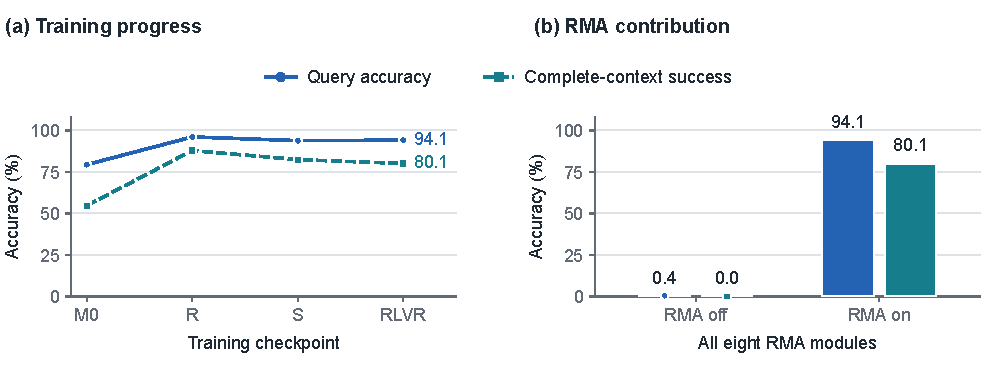
\includegraphics[width=\linewidth]{memory_diagnostic.pdf}
\caption{\textbf{Distant-memory reasoning.} \textbf{(a)} Query accuracy and complete-context success after RMA adaptation (M0), joint adaptation (R), supervised fine-tuning (S), and reinforcement learning with verifiable rewards (RLVR). Complete-context success requires all four answers to be correct. \textbf{(b)} The final model with all eight RMA modules off or on; recurrence and local attention remain active in both settings. With RMA enabled, EdgeRock correctly answers 94.1\% of queries and completes 80.1\% of contexts across retrieval, state updates, cross-document combination, and variable binding.}
\label{fig:memory}
\end{figure}

\subsection{Disabling RMA}
\label{sec:memory-branch-intervention}
All eight RMA modules are disabled at inference time while the recurrent backbone and local attention remain active. Correct answers fall from 964 to 4 of 1,024 queries, and complete-context success from 205 to 0 of 256 contexts (Figure~\ref{fig:memory}). Because RMA is disabled only at inference, this shows that in the trained model, distant answers flow through RMA rather than through recurrence or the local window.

\subsection{Using retained evidence}
\paragraph{Task breakdown.}
EdgeRock-4B achieves 90.6\% complete-context success on exact retrieval, 87.5\% on state-update interpretation, and 89.1\% on cross-document combination (Table~\ref{tab:memory-task-breakdown}).

\paragraph{Paired evidence interventions.}
EdgeRock-4B answers both versions correctly in 89.8\% of 256 pairs where changed distant evidence requires a changed answer, and in 96.5\% of 256 pairs where the answer should stay the same (Table~\ref{tab:paired-memory-interventions}).

\begin{table}[!htbp]
\centering\small
\caption{Memory diagnostics. Top: complete-context success by task, requiring all four answers in a context to be correct (64 contexts per task). Bottom: paired changes to distant evidence, requiring both answers to be correct (256 pairs each); among pairs whose answer should stay the same, the answer never changed.}
\label{tab:memory-task-breakdown}\label{tab:paired-memory-interventions}
\begin{tabularx}{\linewidth}{@{}Yrr@{}}
\toprule
 & Correct / total & Rate (\%)\\
\midrule
\multicolumn{3}{@{}l}{\textit{Complete-context success by task}}\\
Exact retrieval & 58 / 64 & 90.6\\
State-update interpretation & 56 / 64 & 87.5\\
Cross-document combination & 57 / 64 & 89.1\\
Variable binding & 34 / 64 & 53.1\\
All tasks & 205 / 256 & 80.1\\
\addlinespace[4pt]
\multicolumn{3}{@{}l}{\textit{Paired changes to distant evidence}}\\
Answer should change & 230 / 256 & 89.8\\
Answer should stay the same & 247 / 256 & 96.5\\
\bottomrule
\end{tabularx}
\end{table}
